\documentclass[a4paper,article]{memoir}

% Pakker, der skal bruges sideopsætning, billeder m.m.
\usepackage[latin1]{inputenc}
\usepackage[UKenglish]{babel}
%\renewcommand\danishhyphenmins{22}
\usepackage[T1]{fontenc}
\usepackage[margin=3cm]{geometry}
\usepackage{graphicx}
\usepackage{xspace}
\usepackage{color}
\usepackage{array,booktabs}
\usepackage{url}

% Matematik og symboler
\usepackage{amsmath,amssymb}
\usepackage{bm}
\usepackage{amsthm}
\usepackage{mathtools}
\usepackage{listings}
\usepackage{verbatim}

% Fysik pakker
\usepackage{physics}
\usepackage{siunitx}
\usepackage{isotope}

% Pakke der kan lave rette-noter i margin
\usepackage[draft,danish]{fixme}

% ====================================================================
% HUSK AT ÆNDRE TITEL OG FORFATTER
\geometry{headheight=1cm}
\title{\isotope[223]{Ra} gamma spectrum} 	% Dokumentes Titel
\author{Christian Walther Andersen}		% Dokumentets forfatter
%%% \date{i dag}		% Her kan datoen indsættes, men udelades kommandoen indsætter den altid dags dato
% ====================================================================

\begin{document}
	
\setlength{\parindent}{0pt}

\maketitle
\fancybreak{$*\quad*\quad*$}
\vspace{5mm}

% Dokumentet begynder her

\section*{\isotope[223]{Ra} gamma spectrum}

Tab. \ref{tab:spec} lists the photon energies of a selection of the transitions 
observed in the decay products of \isotope[223]{Ra}. The first column shows the 
parent nucleus. The second column shows the observed transition energies of the 
daughter nucleus after the $\alpha$ decay (or $\beta^-$ decay for 
\isotope[211]{Pb}) of the parent. The third column shows the intensity of the 
given transition as a relative frequency for each parent nucleus. Only 
transitions with an energy between 50\si{keV} and 600\si{keV} and an intensity 
of at least 1\% were included.

\begin{table}[h]
\centering
\begin{tabular}{@{}lll@{}}
\toprule
Parent nucleus    & Energy $[\si{keV}]$ & Intensity $\%$ \\ \midrule
\isotope[223]{Ra} & 81.1           & 15             \\
                  & 83.8           & 24             \\
                  & 94.2           & 3              \\
                  & 94.9           & 6              \\
                  & 97.5           & 2              \\
                  & 122            & 1              \\
                  & 144            & 3              \\
                  & 154            & 6              \\
                  & 269            & 14             \\
                  & 324            & 4              \\
                  & 338            & 3              \\
                  & 445            & 1              \\
\isotope[219]{Rn} & 271            & 11             \\
                  & 402            & 7              \\
\isotope[211]{Pb} & 405            & 4              \\
                  & 427            & 2              \\
\isotope[211]{Bi} & 351            & 13             \\ \bottomrule
\end{tabular}
\caption{Spectrum of photon energies emitted by \isotope[223]{Ra} and its decay products.\\Source: https://www.nndc.bnl.gov/nudat2/}
\label{tab:spec}
\end{table}

\section*{Comparison with measurement on NaI-detector}

A measurement of a \isotope[223]{Ra} source with an activity of $\sim 5\si{kBq}$ is shown in Fig. \ref{fig:spec}. The measurement was performed using a NaI-detector gamma camera. The energies from Tab. \ref{tab:spec} are overlaid for comparison.

\begin{figure}[h]
    \centering
    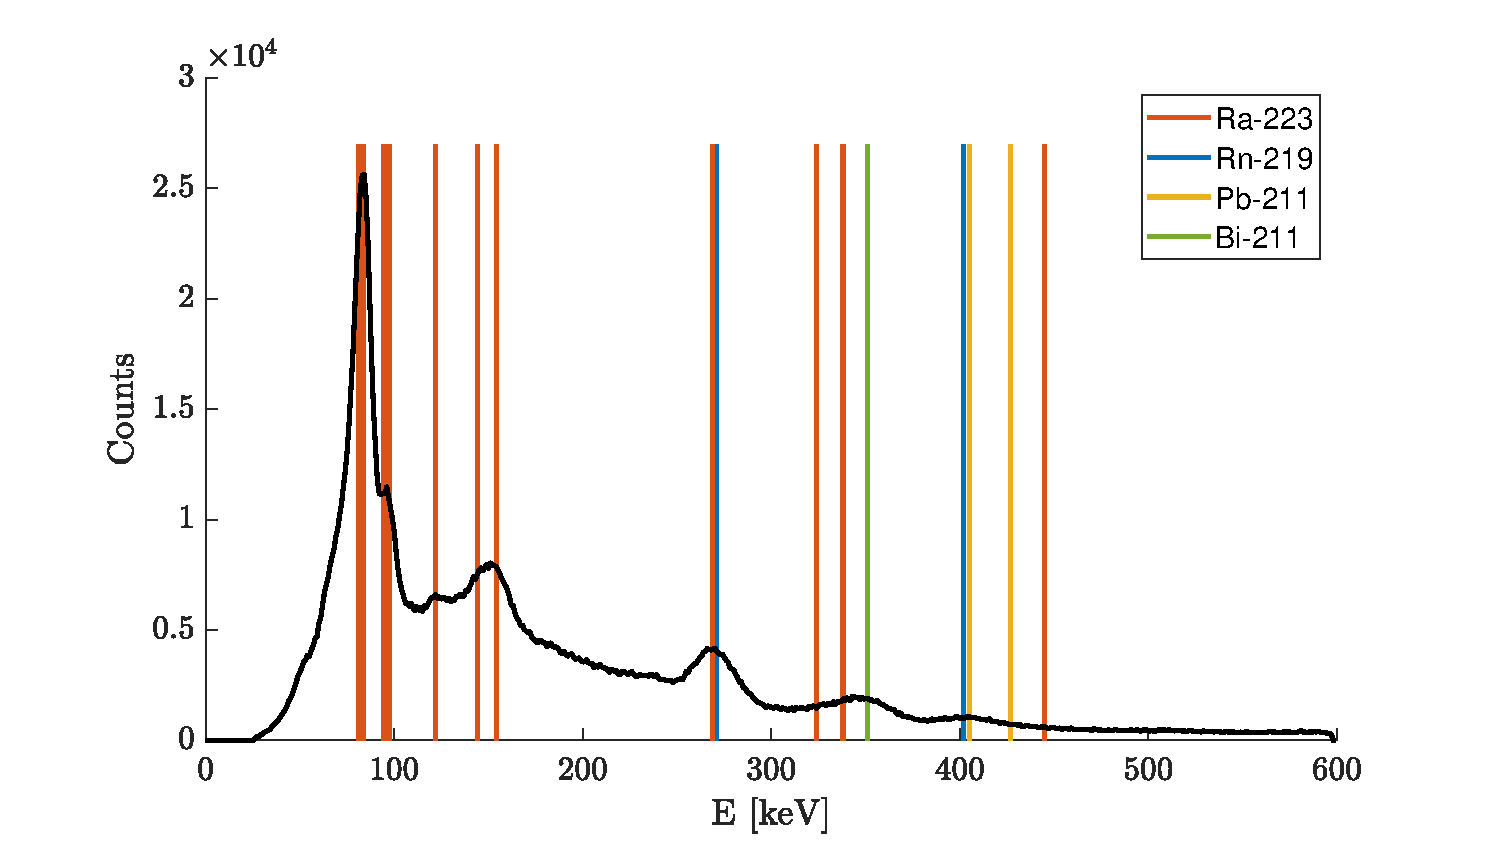
\includegraphics[width=\textwidth]{raspec.eps}
    \caption{Spectrum measured from a \isotope[223]{Ra} source (black line). Energies from Tab. \ref{tab:spec} are shown as lines.}
    \label{fig:spec}
\end{figure}


\section*{Energy windows}

Tab. \ref{tab:windows} shows a prioritised list of energy windows where the 
presence of \isotope[223]{Ra} can be detected. The windows are all 20\% 
windows, however due to the density of the spectrum, multiple transitions are 
included in some of the windows. The windows are prioritised based on the 
minimal detectable activity (MDA), which is estimated from a background 
measurement performed in connection with the measurement of the 
\isotope[223]{Ra} source.

Note that two of the windows overlap.

\begin{table}[h]
	\centering
	\begin{tabular}{@{}ll@{}}
		\toprule
		Window $[\si{keV}]$ & MDA $[\si{Bq}]$ \\ \midrule
		73 - 108            & 18              \\
		130 - 169           & 56              \\
		242 - 298           & 60              \\
		316 - 386           & 90              \\
		360 - 440           & 133             \\ \bottomrule
	\end{tabular}
	\caption{Prioritised list of energy windows in which the presence of 
	\isotope[223]{Ra} can be detected.}
	\label{tab:windows}
\end{table}

\end{document}
